\documentclass[12pt,a4paper,titlepage,final]{report}
\usepackage[utf8]{inputenc}
\usepackage[T1]{fontenc}
\usepackage[slovak]{babel}
\usepackage{times}

\usepackage[unicode,bookmarksopen,pdfpagelabels,colorlinks,plainpages=false,urlcolor=blue,linkcolor=red]{hyperref}

\usepackage{url}
\usepackage{ifpdf}
\usepackage{amsmath}

\ifpdf
  \usepackage[dvipdf]{graphicx}
\else
  \usepackage[dvips]{graphicx}
\fi

\usepackage[top=2cm, left=2cm, text={17cm, 26cm}, ignorefoot]{geometry}

\begin{document}

\begin{titlepage}

% \vspace*{1cm}
\begin{figure}[!h]
  \centering
  \includegraphics[height=5cm]{img/logo}
\end{figure}

\vfill

\begin{center}
\begin{Large}
Dokumentace k projektu pro předměty IZP a IUS\\
\end{Large}
\bigskip
\begin{Huge}
Iterační výpočty\\
\end{Huge}
\smallskip
\begin{large}
projekt č. 2
\end{large}
\end{center}

\vfill

\begin{center}
\begin{Large}
\today
\end{Large}
\end{center}

\vfill

\begin{flushleft}
\begin{large}
\begin{tabular}{ll}
Autor: & Ján Mochňak, \url{xmochn00@stud.fit.vutbr.cz} \\
 & Fakulta Informačních Technologií \\
 & Vysoké Učení Technické v Brně \\
\end{tabular}
\end{large}
\end{flushleft}
\end{titlepage}


\pagestyle{plain}
\pagenumbering{roman}
\setcounter{page}{1}
\tableofcontents

\newpage
\pagestyle{plain}
\pagenumbering{arabic}
\setcounter{page}{1}

\chapter{Úvod} \label{uvod}
Dokumentácia k druhému projektu do predmetov \textit{základy programovania} a \textit{softwérové inžinierstvo}, ktoré sa vyučujú na VUT v Brně.

Výsledkom projektu je konzolová aplikácia napísana v jazyku \textit{C}, splňujúca štandard \textit{C99}. Aplikácia má dve hlavné úlohy, jednou z nich je overenie správnosti implementácie matematickej funkcie \textit{tangens} pomocou \textit{Taylorového rozvoja} a pomocou \textit{zreťazených zlomkov}. Tieto funkie sú implementované len pomocou základných matematických operácii. Druhá úloha tejto aplikácie spočíva vo výpočte vzdialenosti a výšky meraného objektu, v ktorej nájdeme využitie funkie \textit{tangens}.


\chapter{Analýza problému} \label{analyza}
Pre výpočet vzdialeností budeme potrebovať funkciu tangens, takže sa na možnosti implementácie tejto funckie pozrieme bližšie.

\section{Zadanie problému}
Hlavnou úlohou je vypočítanie vzdialenosti a výšky meraného objektu, predpokladáme, že merací prístroj má možnosť nastavenia aj jeho výšky. Grafické zobrazenie tohoto problému je v obrázku \ref{fig:pajko}.

\begin{figure}[!h]
  \centering
  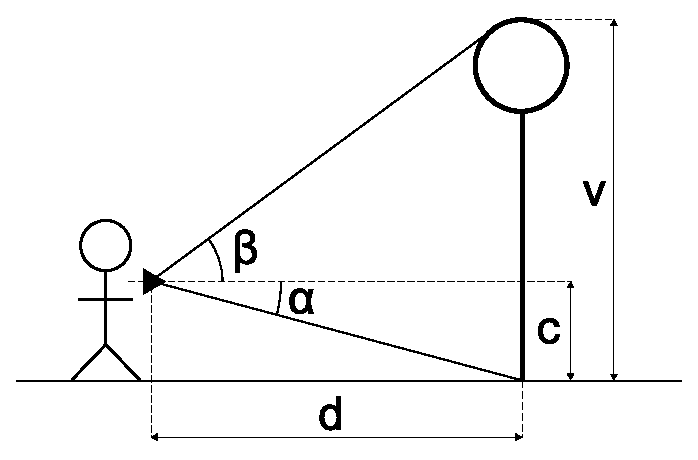
\includegraphics[scale=0.75]{img/drawing}
	\caption{Náčrtok meracieho zariadenia a meraného objektu.}
  \label{fig:pajko}
\end{figure}

\section{Možnosti výpočtu funkie tan}
Matematicky je funkcia tan definovaná ako:
\begin{equation} \label{eq:taylor}
\tan(x) = \frac{\sin(x)}{\cos(x)}
\end{equation}

Ak by sme chceli teda vypočítať tangens úhla x, potrebovali by sme k tomu ešte aj funkie sínus a cosínus. A preto sa pozrieme na ďalšie možné výpočty.

\subsection{Taylorov rozvoj}
Taylorov rozvoj by sme dokázali vyjadriť takto:
\begin{equation} \label{eq:taylor}
\tan(x) = x + \frac{x^3}{3} + \frac{2x^5}{15} + \frac{17x^7}{315} + \frac{62x^9}{2835} + ...
\end{equation}

Pričom v našom prípade rátame len s prvými 13 členmy Taylorovej rady, pre čitateľov \cite{numerators} a menovateľov \cite{denominators}, boli využité overené online zdroje. Maximálny počet iterácii pre spresnenie výsledku je v tomto prípade len 13.

\subsection{Zreťazenie zlomkov} \label{subsec:zlomky}
Fuknciu tangens pomocou zreťazenia zlomkov, vyjadríme takto:
\begin{equation} \label{eq:cfrac}
\tan(x) = \cfrac{1}{ \cfrac{1}{x} - \cfrac{1}{\cfrac{3}{x} - \cfrac{1}{\cfrac{5}{x} - \cfrac{1}{\cfrac{7}{x} - ... }} }}
\end{equation}

Výhodou tejto možnosti je hlavne možnosť viacero iterácii a teda vyššiej presnosti ako u Taylorového rozvoja. A z tohto dôvodu volíme, pre výpočet výšky a vzdialenosti meraného objektu túto funkciu.

\chapter{Návrh riešenia problému}
Po analýze funkcie tangens, som sa rozhodol akceptovať len hodnoty \texttt{0 < $\alpha$ <= 1.4 rad}, ktoré sa nachadzajú v prvom kvadrante. Toto obmedzenie je pre naše účely dostačujúce, hodnota úhlov $\alpha$ a $\beta$ by podľa obrázku \ref{fig:pajko} nemala presiahnúť $90^\circ$.

\section{Porovnanie presností výpočtov tangens}
Pri porovnávaní je potrebné zistit ako sa veľmi sa odchyľuje výsledok iterácií z našich implementácií funkcie tangens oproti funkcii \textit{tan} z matematickej knižnice \texttt{<math.h>}. Rozdielom výsledkov je vyjadrená absolútna odchýlka pre každú iteráciu, ale aj funkciu.

\section{Výpočet vzdialenosti a výšky meraného objektu}
Ako implicitnú výšku zariadenia volíme 1.5, ktorá je definovaná zadaním. Pre výpočty použijeme definíciu tan v následujúcom tvare:
\begin{equation}
\tan(\alpha)=\frac{a}{b}=\frac{\text{protiľahlá}}{\text{priľahlá}}
\end{equation}

Inými slovami $\tan(\alpha)$ je pomer dĺžok odvesny protiľahlej k tomuto uhlu a dĺžky odvesny k nemu priľahlej.

Presnosť, resp. počet iterácií sme si zvolili 11, pretože po tejto iterácii je výsledok pre datový typ \texttt{double} rovnaký. Tým sme dosiahli najvyššiu možnú presnosť.

\subsection{Výpočet vzdialenosti} \label{subsec:vypocet_vzdialenost}
Vzdialenosť objektu od meracieho prístroja si z obrázku \ref{fig:pajko} vyjadríme takto:
\begin{equation}
\tan(\alpha)=\frac{c}{d} \Rightarrow d=\frac{c}{\tan(\alpha)}
\end{equation}

Pri výpočte $\tan(\alpha)$ využijeme metódu zreťazených zlomkov (viz. \ref{subsec:zlomky}).

\subsection{Výpočet výšky}
Výšku meraného objektu si vieme opäť odvodiť z obrázka \ref{fig:pajko}:
\begin{equation}
\tan(\beta)=\frac{v_1}{d} \Rightarrow v = c + \tan(\beta) * d
\end{equation}

K výslednej výške je potreba pripočítať výšku zariadenia $c$. Pri výpočte $\tan(\beta)$ využijeme metódu zreťazených zlomkov (viz. \ref{subsec:zlomky}). Pre tento výpočet si musíme najprv vypočítať jeho vzdialenosť $d$ pomocou \ref{subsec:vypocet_vzdialenost}.

\chapter{Špecifikácia testov}

\paragraph{Test 1:} Chybná syntaxe $\longrightarrow$ Detekce chyby.
\begin{verbatim}
./proj2               ; nedostatok parametrov
./proj2 -tan          ; správne -tan
./proj2 -m            ; je potrebné zadať hodnotu úhlu
./proj2 -m -c 2.2     ; výška musí byť nastavená pred úhlami
./proj2 -c 2.2        ; potreba nastaviť hodnotu úhlu -m
\end{verbatim} 

\paragraph{Test 2:} Nesmyslná syntaxe $\longrightarrow$ Detekce chyby.
\begin{verbatim}
./proj2 --tan 5 1 10        ; úhol nieje z intervalu <0,1.4>
./proj2 --tan 0.165461 1 52 ; maximálny počet iterácií je 13
./proj2 -c 233 -m 1.2       ; maximálna výška 100
\end{verbatim} 

\paragraph{Test 3:} Porovnanie výpočtov $\longrightarrow$ Predpokladaný výstup.
\begin{verbatim}
./proj2 --tan 1.024 10 10
10 1.642829e+00 1.642552e+00 2.773337e-04 1.642829e+00 0.000000e+00

./proj2 --tan 0.785398163 10 10
10 1.000000e+00 9.999992e-01 8.095039e-07 1.000000e+00 1.110223e-16
\end{verbatim}

\paragraph{Test 4:} Výpočet vzdialenosti a výšky $\longrightarrow$ Predpokladaný výstup.
\begin{verbatim}
./proj2 -m 0.3
4.8490922156e+00
7.6106234032e+00

./proj2 -m 0.3 0.9
4.8490922156e+00
7.6106234032e+00

./proj2 -c 1.7 -m 0.15 1.3
1.1248205560e+01
4.2217188781e+01
\end{verbatim} 

\chapter{Popis riešenia}

\section{Analýza vstupných parametrov}
Pre overenie správnosti zadania číselných hodnôt sú použité funkcie \texttt{strtod} a \texttt{strdol}, ktoré viedlo k zjednodušeniu kódu.

\section{Ovládanie programu}
Program obsahuje nápovedu, ktorú vyvoláme parametrom \texttt{--help}. Nápoveda obsahuje presné informácie o vstupných parametroch, ktoré určujú funkciu programu.

Všetky chybné výstupy sa zobrazujú do štadardného chybového výstupu, validné výstupu sa zobrazujú do štandardného výstupu.

\section{Implementácia}
Parametry z príkazového riadka spracováva funkcia \texttt{parse\_args}, ktorá naplní štruktúru \texttt{params}. Následne podľa tejto štruktúry rozvetvíme program na dve časti, jedna z nich spracováva parameter \texttt{--tan} a druhá \texttt{-m}.

Pri výpočtoch odchýlky používame funkciu \texttt{show\_tan\_diff\_table}, ktorá postupne iteruje a zobrazuje výsledky na štandardný výstup. Implementáciu Tayloroveho rozvoja nájdeme vo funkci \texttt{taylor\_tan} a metódu zreťazených zlomkov \texttt{cfrac\_tan}.

Pre výpočet vzdialenosti použivame funkciu \texttt{calculate\_distance} a výsledok z nej zobrazíme na štandardný výstup. Pre výpočet výšky objektu je použitá funkcia \texttt{calculate\_height}, predtým je však potreba overiť, či bol zadaný aj úhol $\beta$, kedže je tento parameter voliteľný. Výsledok je následne vypísaný na štandardný výstup.

Ak v tomto priebehu nastena chyba, (napr. nevalidné hodnoty parametrov) nastavíme hodnotu premennej \texttt{err} a následne zavoláme funkciu \texttt{show\_error\_and\_halt}, ktorá program ukonči s chybovou hláškou.

\chapter{Záver}
Aplikácia vypočíta vzdialenosť a výšku objektu pomocou vytvorenej funkie tangens. Pre výpočet bola použitá metóda zreťazenia zlomkov (viď \ref{subsec:zlomky}), hlavne z dôvodu väčšiej presnosti. Program splňuje všetky požiadavky uvedené v zadaní a taktiež funguje pre všetky testovacie prípady.

Pre naše účeli sme obmedzili veľkosť vstupného úhla na prvý kvadrant, toto obmedzenie by mohli riešiť vyššie verzie programu. Pre aktuálnu činnosť to však nieje potrebné.

Program bol úspešne otestovaný na platformách Linux a Windows 32-bit. Nieje potrebné vytváť akúkoľvek zmenu v kóde pre jeho správnu kompiláciu, avšak je potrebné mať na platforme definované 64-bit číslo (uint64\_t).

\bibliographystyle{plain}
\bibliography{ius2}

\appendix
\chapter{Metriky kódu} \label{metriky}
\paragraph{Počet súborov:} 1 súbor
\paragraph{Počet riadkov zdrojového textu:} 282 riadkov
\paragraph{Veľkosť statických dát:} 6739B
\paragraph{Veľkosť spustiteľného súbora:} 11.5kB (Windows 32-bit, pri preklade bez ladiacich informácií)

\end{document}